\PassOptionsToPackage{unicode=true}{hyperref} % options for packages loaded elsewhere
\PassOptionsToPackage{hyphens}{url}
%
\documentclass[english,man,floatsintext]{apa6}
\usepackage{lmodern}
\usepackage{amssymb,amsmath}
\usepackage{ifxetex,ifluatex}
\usepackage{fixltx2e} % provides \textsubscript
\ifnum 0\ifxetex 1\fi\ifluatex 1\fi=0 % if pdftex
  \usepackage[T1]{fontenc}
  \usepackage[utf8]{inputenc}
  \usepackage{textcomp} % provides euro and other symbols
\else % if luatex or xelatex
  \usepackage{unicode-math}
  \defaultfontfeatures{Ligatures=TeX,Scale=MatchLowercase}
\fi
% use upquote if available, for straight quotes in verbatim environments
\IfFileExists{upquote.sty}{\usepackage{upquote}}{}
% use microtype if available
\IfFileExists{microtype.sty}{%
\usepackage[]{microtype}
\UseMicrotypeSet[protrusion]{basicmath} % disable protrusion for tt fonts
}{}
\IfFileExists{parskip.sty}{%
\usepackage{parskip}
}{% else
\setlength{\parindent}{0pt}
\setlength{\parskip}{6pt plus 2pt minus 1pt}
}
\usepackage{hyperref}
\hypersetup{
            pdftitle={The MeloSol Corpus},
            pdfkeywords={melodic corpus, Tonal music, kern, sight singing},
            pdfborder={0 0 0},
            breaklinks=true}
\urlstyle{same}  % don't use monospace font for urls
\usepackage{graphicx,grffile}
\makeatletter
\def\maxwidth{\ifdim\Gin@nat@width>\linewidth\linewidth\else\Gin@nat@width\fi}
\def\maxheight{\ifdim\Gin@nat@height>\textheight\textheight\else\Gin@nat@height\fi}
\makeatother
% Scale images if necessary, so that they will not overflow the page
% margins by default, and it is still possible to overwrite the defaults
% using explicit options in \includegraphics[width, height, ...]{}
\setkeys{Gin}{width=\maxwidth,height=\maxheight,keepaspectratio}
\setlength{\emergencystretch}{3em}  % prevent overfull lines
\providecommand{\tightlist}{%
  \setlength{\itemsep}{0pt}\setlength{\parskip}{0pt}}
\setcounter{secnumdepth}{0}

% set default figure placement to htbp
\makeatletter
\def\fps@figure{htbp}
\makeatother

% Manuscript styling
\usepackage{upgreek}
\captionsetup{font=singlespacing,justification=justified}

% Table formatting
\usepackage{longtable}
\usepackage{lscape}
% \usepackage[counterclockwise]{rotating}   % Landscape page setup for large tables
\usepackage{multirow}		% Table styling
\usepackage{tabularx}		% Control Column width
\usepackage[flushleft]{threeparttable}	% Allows for three part tables with a specified notes section
\usepackage{threeparttablex}            % Lets threeparttable work with longtable

% Create new environments so endfloat can handle them
% \newenvironment{ltable}
%   {\begin{landscape}\begin{center}\begin{threeparttable}}
%   {\end{threeparttable}\end{center}\end{landscape}}
\newenvironment{lltable}{\begin{landscape}\begin{center}\begin{ThreePartTable}}{\end{ThreePartTable}\end{center}\end{landscape}}

% Enables adjusting longtable caption width to table width
% Solution found at http://golatex.de/longtable-mit-caption-so-breit-wie-die-tabelle-t15767.html
\makeatletter
\newcommand\LastLTentrywidth{1em}
\newlength\longtablewidth
\setlength{\longtablewidth}{1in}
\newcommand{\getlongtablewidth}{\begingroup \ifcsname LT@\roman{LT@tables}\endcsname \global\longtablewidth=0pt \renewcommand{\LT@entry}[2]{\global\advance\longtablewidth by ##2\relax\gdef\LastLTentrywidth{##2}}\@nameuse{LT@\roman{LT@tables}} \fi \endgroup}

% \setlength{\parindent}{0.5in}
% \setlength{\parskip}{0pt plus 0pt minus 0pt}

% \usepackage{etoolbox}
\makeatletter
\patchcmd{\HyOrg@maketitle}
  {\section{\normalfont\normalsize\abstractname}}
  {\section*{\normalfont\normalsize\abstractname}}
  {}{\typeout{Failed to patch abstract.}}
\makeatother
\shorttitle{MeloSol}
\author{David John Baker\textsuperscript{1}}
\affiliation{
\vspace{0.5cm}
\textsuperscript{1} Louisiana State University}
\authornote{David John Baker now works at Flatiron School in London, England


Correspondence concerning this article should be addressed to David John Baker, . E-mail: davidjohnbaker1@gmail.com}
\keywords{melodic corpus, Tonal music, kern, sight singing\newline\indent Word count: ~900}
\usepackage{lineno}

\linenumbers
\usepackage{csquotes}
\ifnum 0\ifxetex 1\fi\ifluatex 1\fi=0 % if pdftex
  \usepackage[shorthands=off,main=english]{babel}
\else
  % load polyglossia as late as possible as it *could* call bidi if RTL lang (e.g. Hebrew or Arabic)
  \usepackage{polyglossia}
  \setmainlanguage[]{english}
\fi

\title{The MeloSol Corpus}

\date{}

\abstract{
This paper introduces the \emph{MeloSol} corpus, a collection of 783 Western, tonal monophonic melodies. We first begin by describing the overal structure of the corpus, then proceede to detail its contents as they would be helpful for researchers working in the field of computational musicology or music psychology. In order to contextualizs the MeloSol corpus in relation to other corpora in the literature, we present descriptive statistics of the \emph{MeloSol} corpus alongside the \emph{The Densmore Collection of Native American Song} and \emph{The Essen Folk Song Collection}. We suggest posible futures uses of this corpus including extending research investigating Western tonality, perceptual experiments neededing novel ecological stimuli, or work involving the musical generation of monophonic melodies in the style of Western tonal music.
}

\begin{document}
\maketitle

\hypertarget{introdution}{%
\section{Introdution}\label{introdution}}

This data report introduces the \emph{MeloSol} corpus, a collection of 783 monophonic melodies taken from \emph{A New Approach to Sight Singing: Fifth Edition} (Berkowitz, Fontrier, Kraft, Goldstein, \& Smaldone, 2011).
The title \emph{MeloSol} derives from a combination of the corpus' content-- \emph{Melo} dic data-- and the first name of the original author of the collection, \emph{Sol} Berkowitz.

The corpus is divided into two major sections: a collection of sight singing melodies composed specifically for pedagogical purposes (n = 629) taken from Chapter One and examples from Western Classical literature (n = 154) taken from Chapter Five.
The original text also contains materials for practicing rhythm (Chapter Two), Singing Duets (Chapter Three), Sing and Plays that incoproate a melody and piano accompaniament (Chapter Four), and Supplementary Exercises that are not included here.
Within each of the larger sections exists five further subdivisions.
These five subdivisions are mapped in conjunction with the trajectory of many aural skills classrooms.

For example, the first section of both the sight singing melodies and the first section of literature align with melodies a first semester undergraduate student in a music degree program might be expected to learn during their first semester of university in an aural skills classroom.
As the original book was designed as a pedaogical text, each section of the book and consequently each melody within each section is meant to increase in complexity as new topics are introduced.
The fifth and final section of both the sight singing melodies and examples from the literature contains melodies which break from Western tonal practice.
These melodies contain either modal, atonal, or tonally ambigious melodies.
A visual depitction of the breakdown of melodies from the two larger sections in terms of count data is presented in FIGURE ONE.
In terms of analyzable data, the 783 melodies are encoded in \texttt{**kern} format (Huron, 1994), with each individual file containing metadata listing the unique identifier, chapter from which the melody originates, section within that chapter of the larger text, page number, as well as what mode the encoder labeled the melody as.
Modes were only noted for a small subset of the corpus, the vast majority of these melodies are either major (ionian) or minor (aeolean).
Other corpora should be consulted for questions pertaining to mode such as work by Albrecht and Huron (Albrecht \& Huron, 2014).

Overall, the corpus consists of 49,730 \texttt{**kern} tokens, a subset of which are 36,641 note heads.
All melodies in the corpus were encoded by hand using the software MuseScore (Werner, Nicholas, \& Bonte, 2019), initially saved as XML, then converted to \texttt{**kern} using the humdrum extras \texttt{xml2hum} tool (Sapp, 2008) with the current meta data added using the \texttt{metadata\_adder.R}.
Further addition to the metadata can be added with modifications to \texttt{metadat\_adder.R} found in the \texttt{scripts/R} directory.
We describe the corpus from a macro perspective in Figure XXXX.
Section V was removed from the top left portion of Figure XXX as the majority of melodies in the atonal section of the corpus are encoded with a zero flat, zero sharp key signature and that including those in the figure would skew C major and A minor's representitivness.

\begin{figure}
\centering
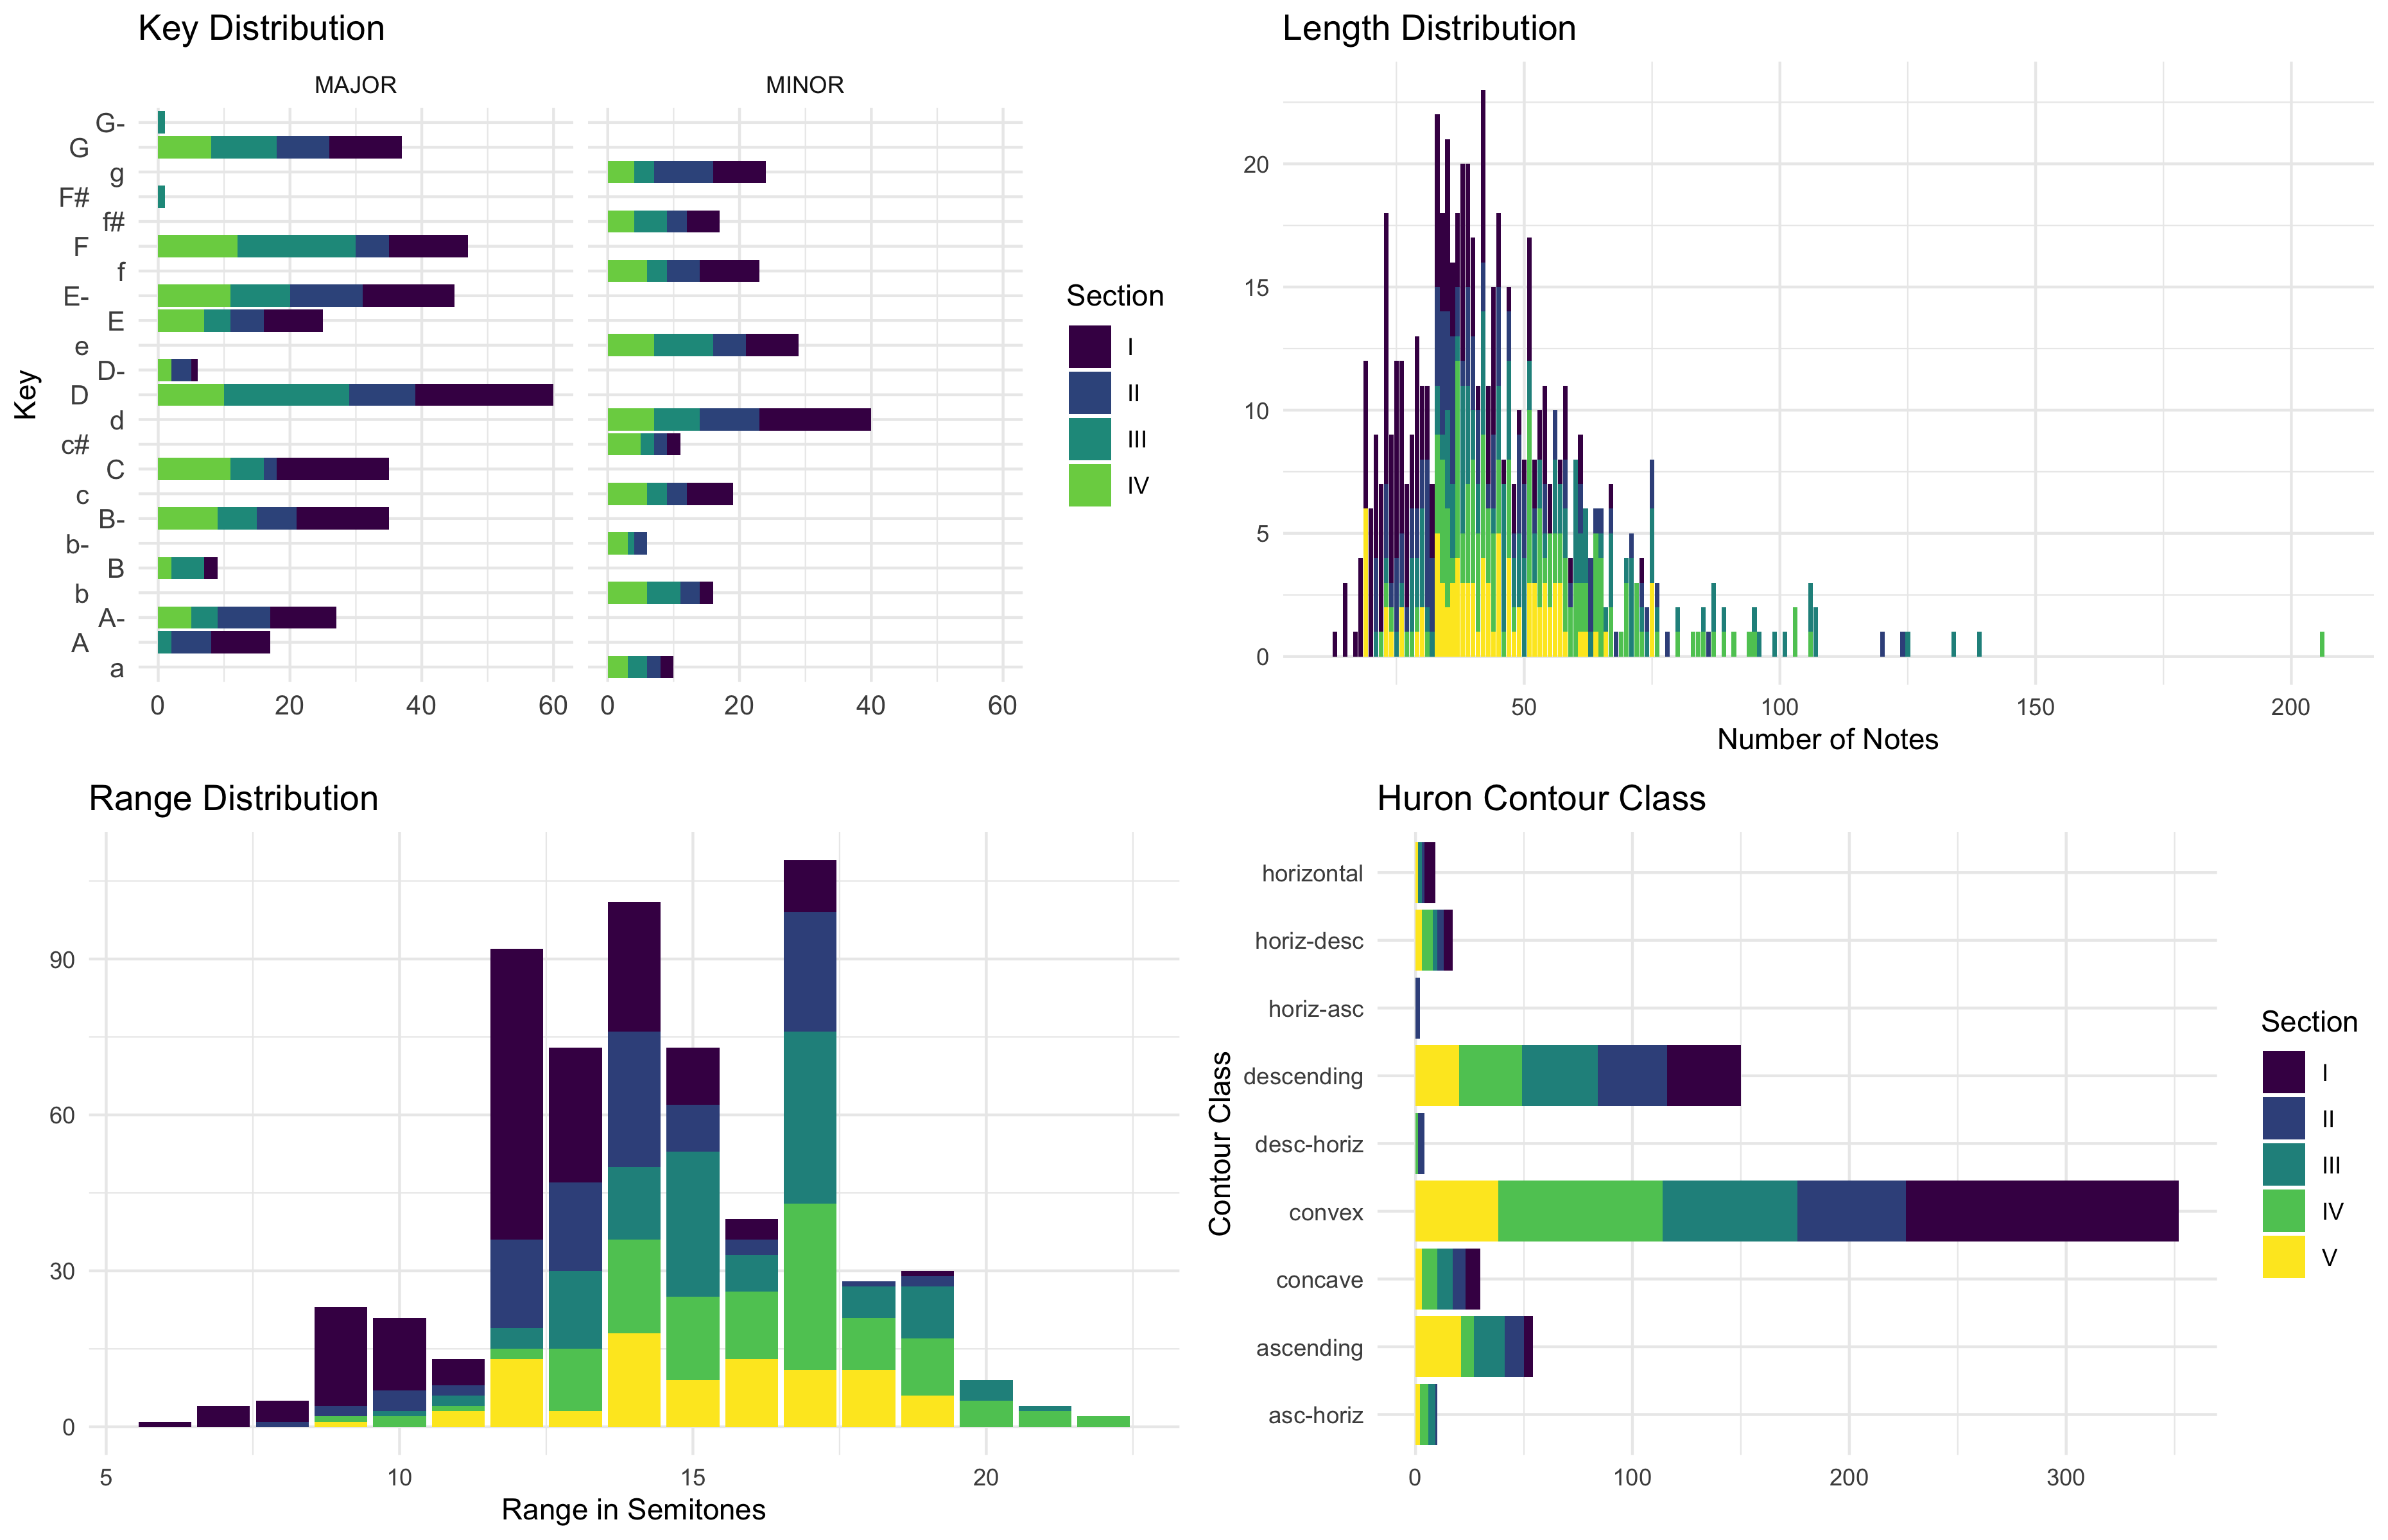
\includegraphics{../img/descriptive_panel.png}
\caption{Descriptive Statistics of MeloSol}
\end{figure}

\hypertarget{comparison}{%
\section{Comparison}\label{comparison}}

In order to further contextualize the \emph{MeloSol} corpus with the context of other corpora found in the literature, we briefly compare descriptive statistics from the \emph{MeloSol} corpus with both \emph{The Densmore Collection of Native American Songs} (Neubarth, Shanahan, \& Conklin, 2018; Shanahan \& Shanahan, 2014) as well as the European and Chinese subset of the \emph{Essen Folk Song Collection} (Schaffrath, 1995).
We chose both the \emph{Densmore} as well as the \emph{Essen} collection seeing as both corpora contain monophonic melodies.
Further, we compare the \emph{MeloSol} with the \emph{Essen} collection as the \emph{Essen} collection has been used as a proxy for representing the implicit understanding of the structure of Western, tonal music in computational models that depend theoretically on the concept of implicit, statistical learning (Demorest \& Morrison, 2016; Huron, 2006; Pearce, 2018).
Comparisons of descriptive statistics were conducted using the FANTASTIC toolbox (Mullensiefen, 2009).
The accompanying calculations for each melody are found in \texttt{corpus/melosol\_fantastic\_features.csv}.

\begin{figure}
\centering
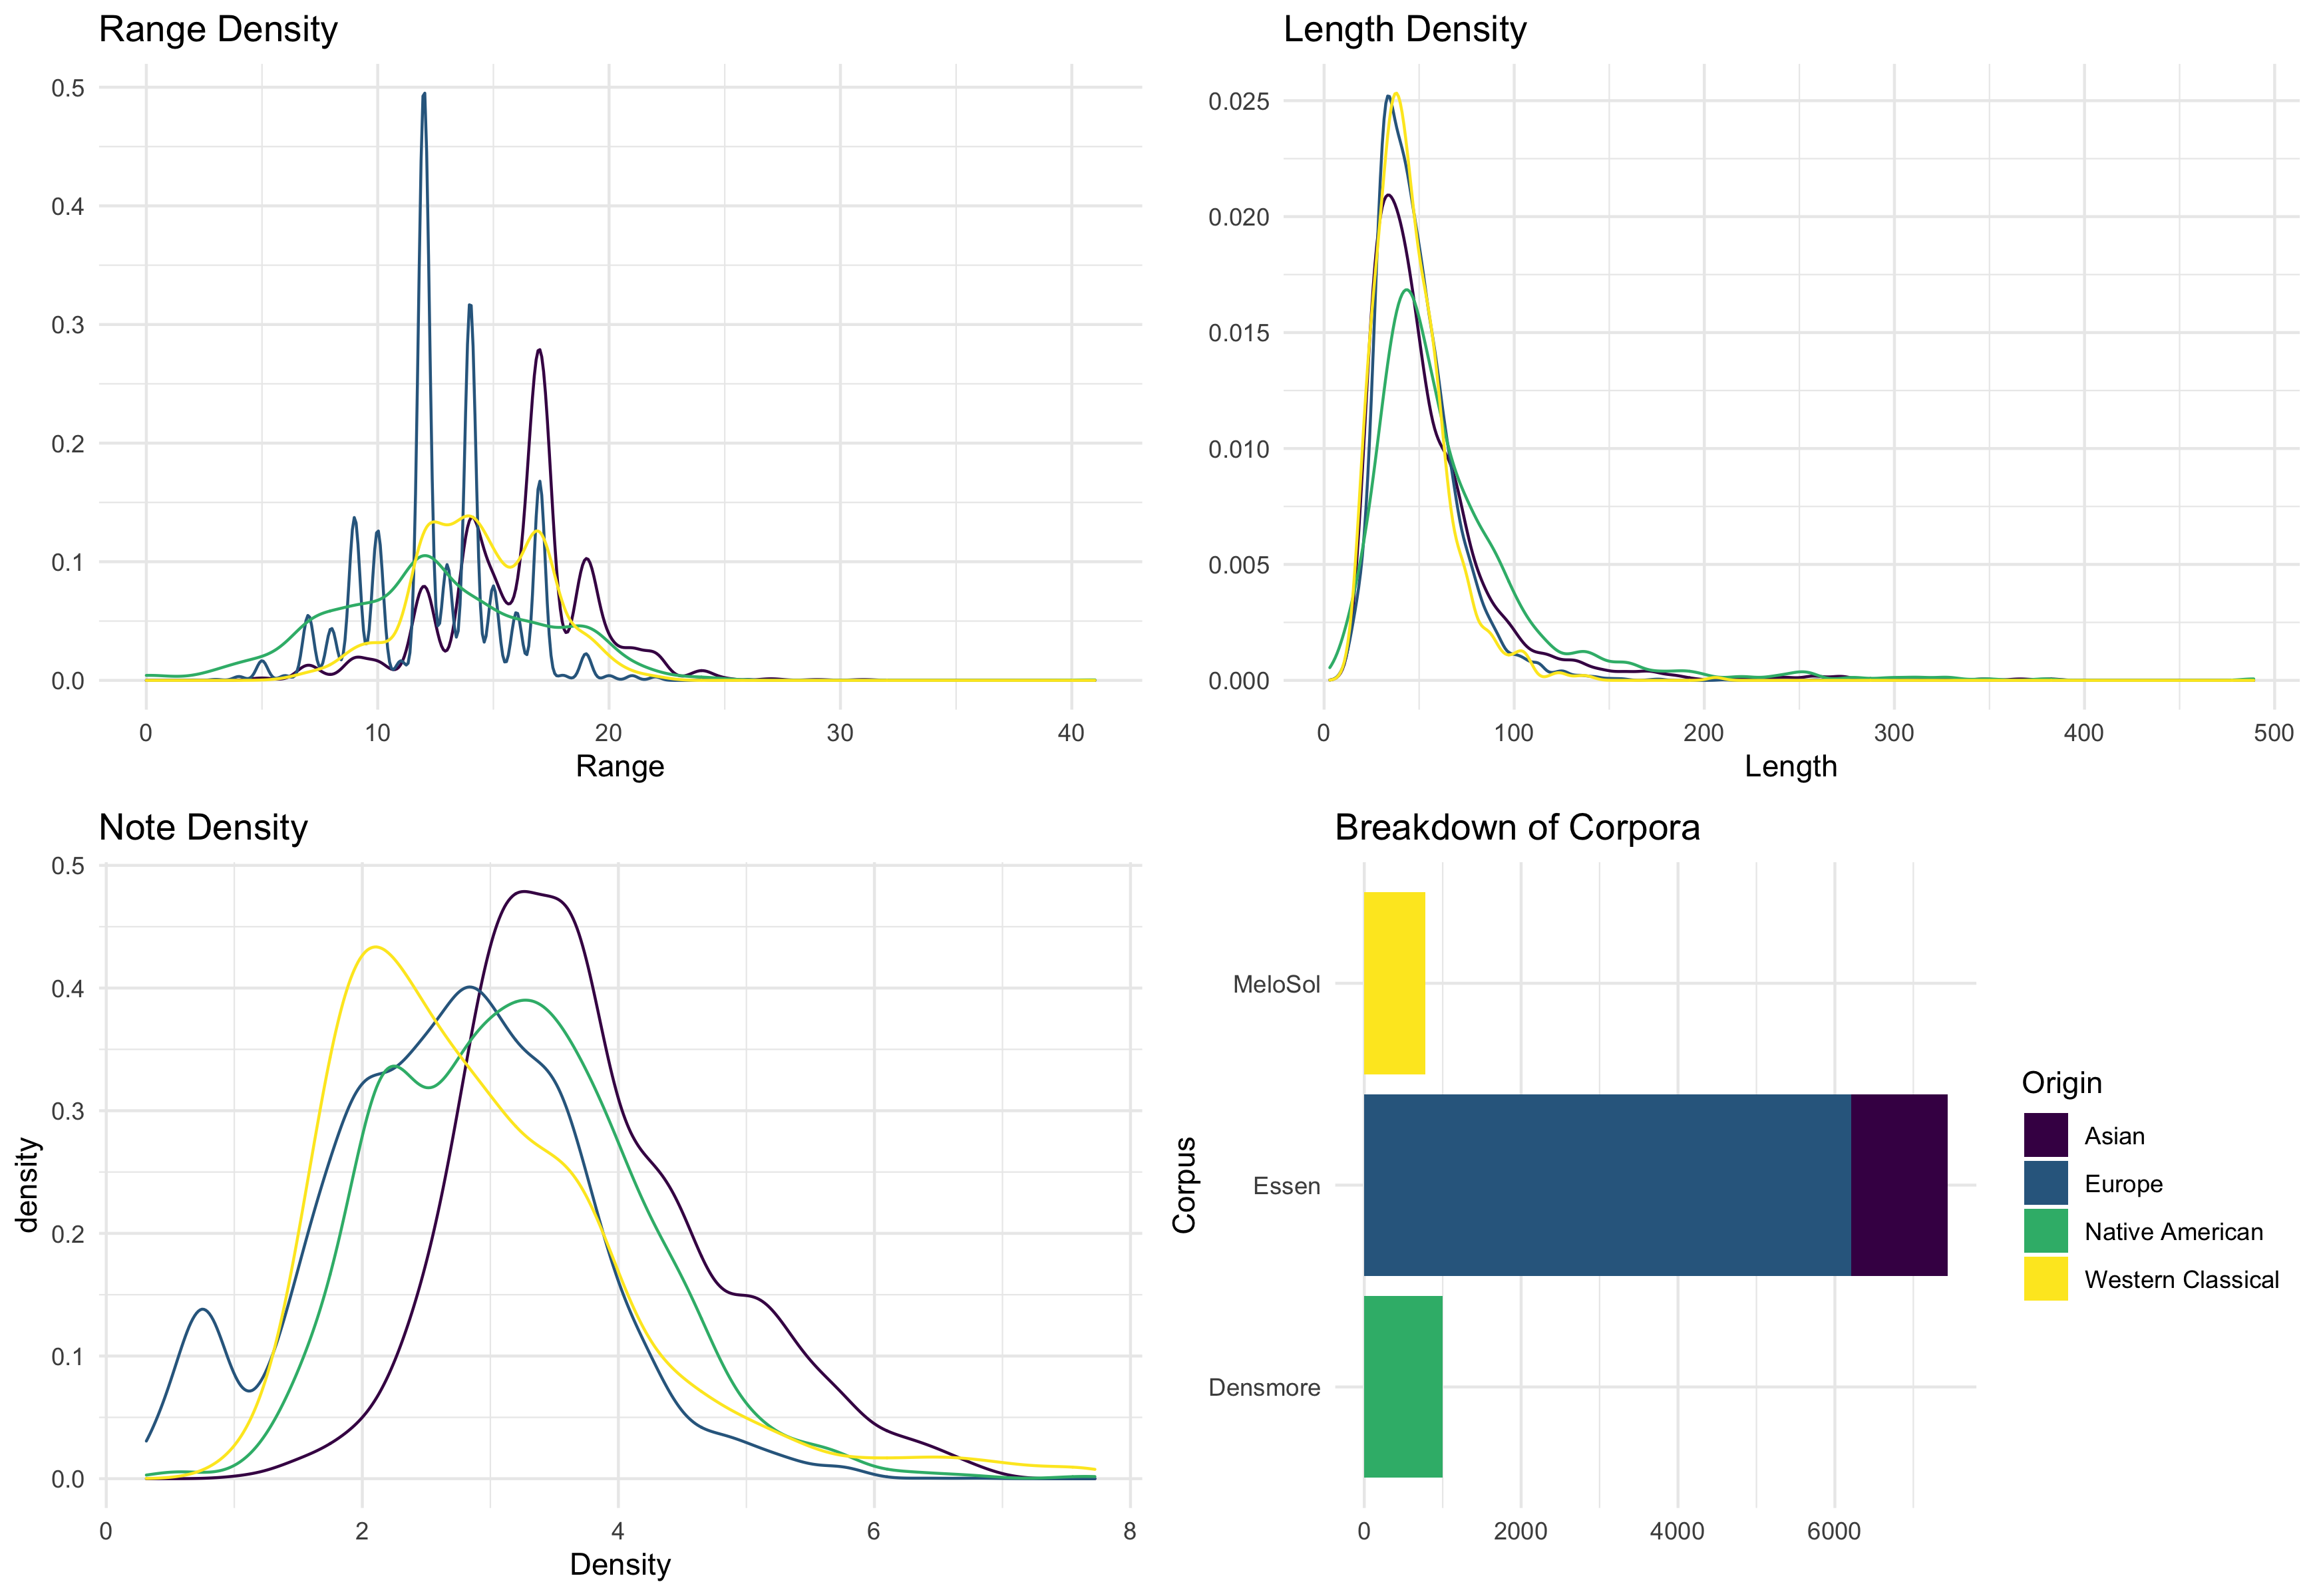
\includegraphics{../img/comparative_descriptive_panel.png}
\caption{Descriptive Statistics of MeloSol}
\end{figure}

\begin{figure}
\centering
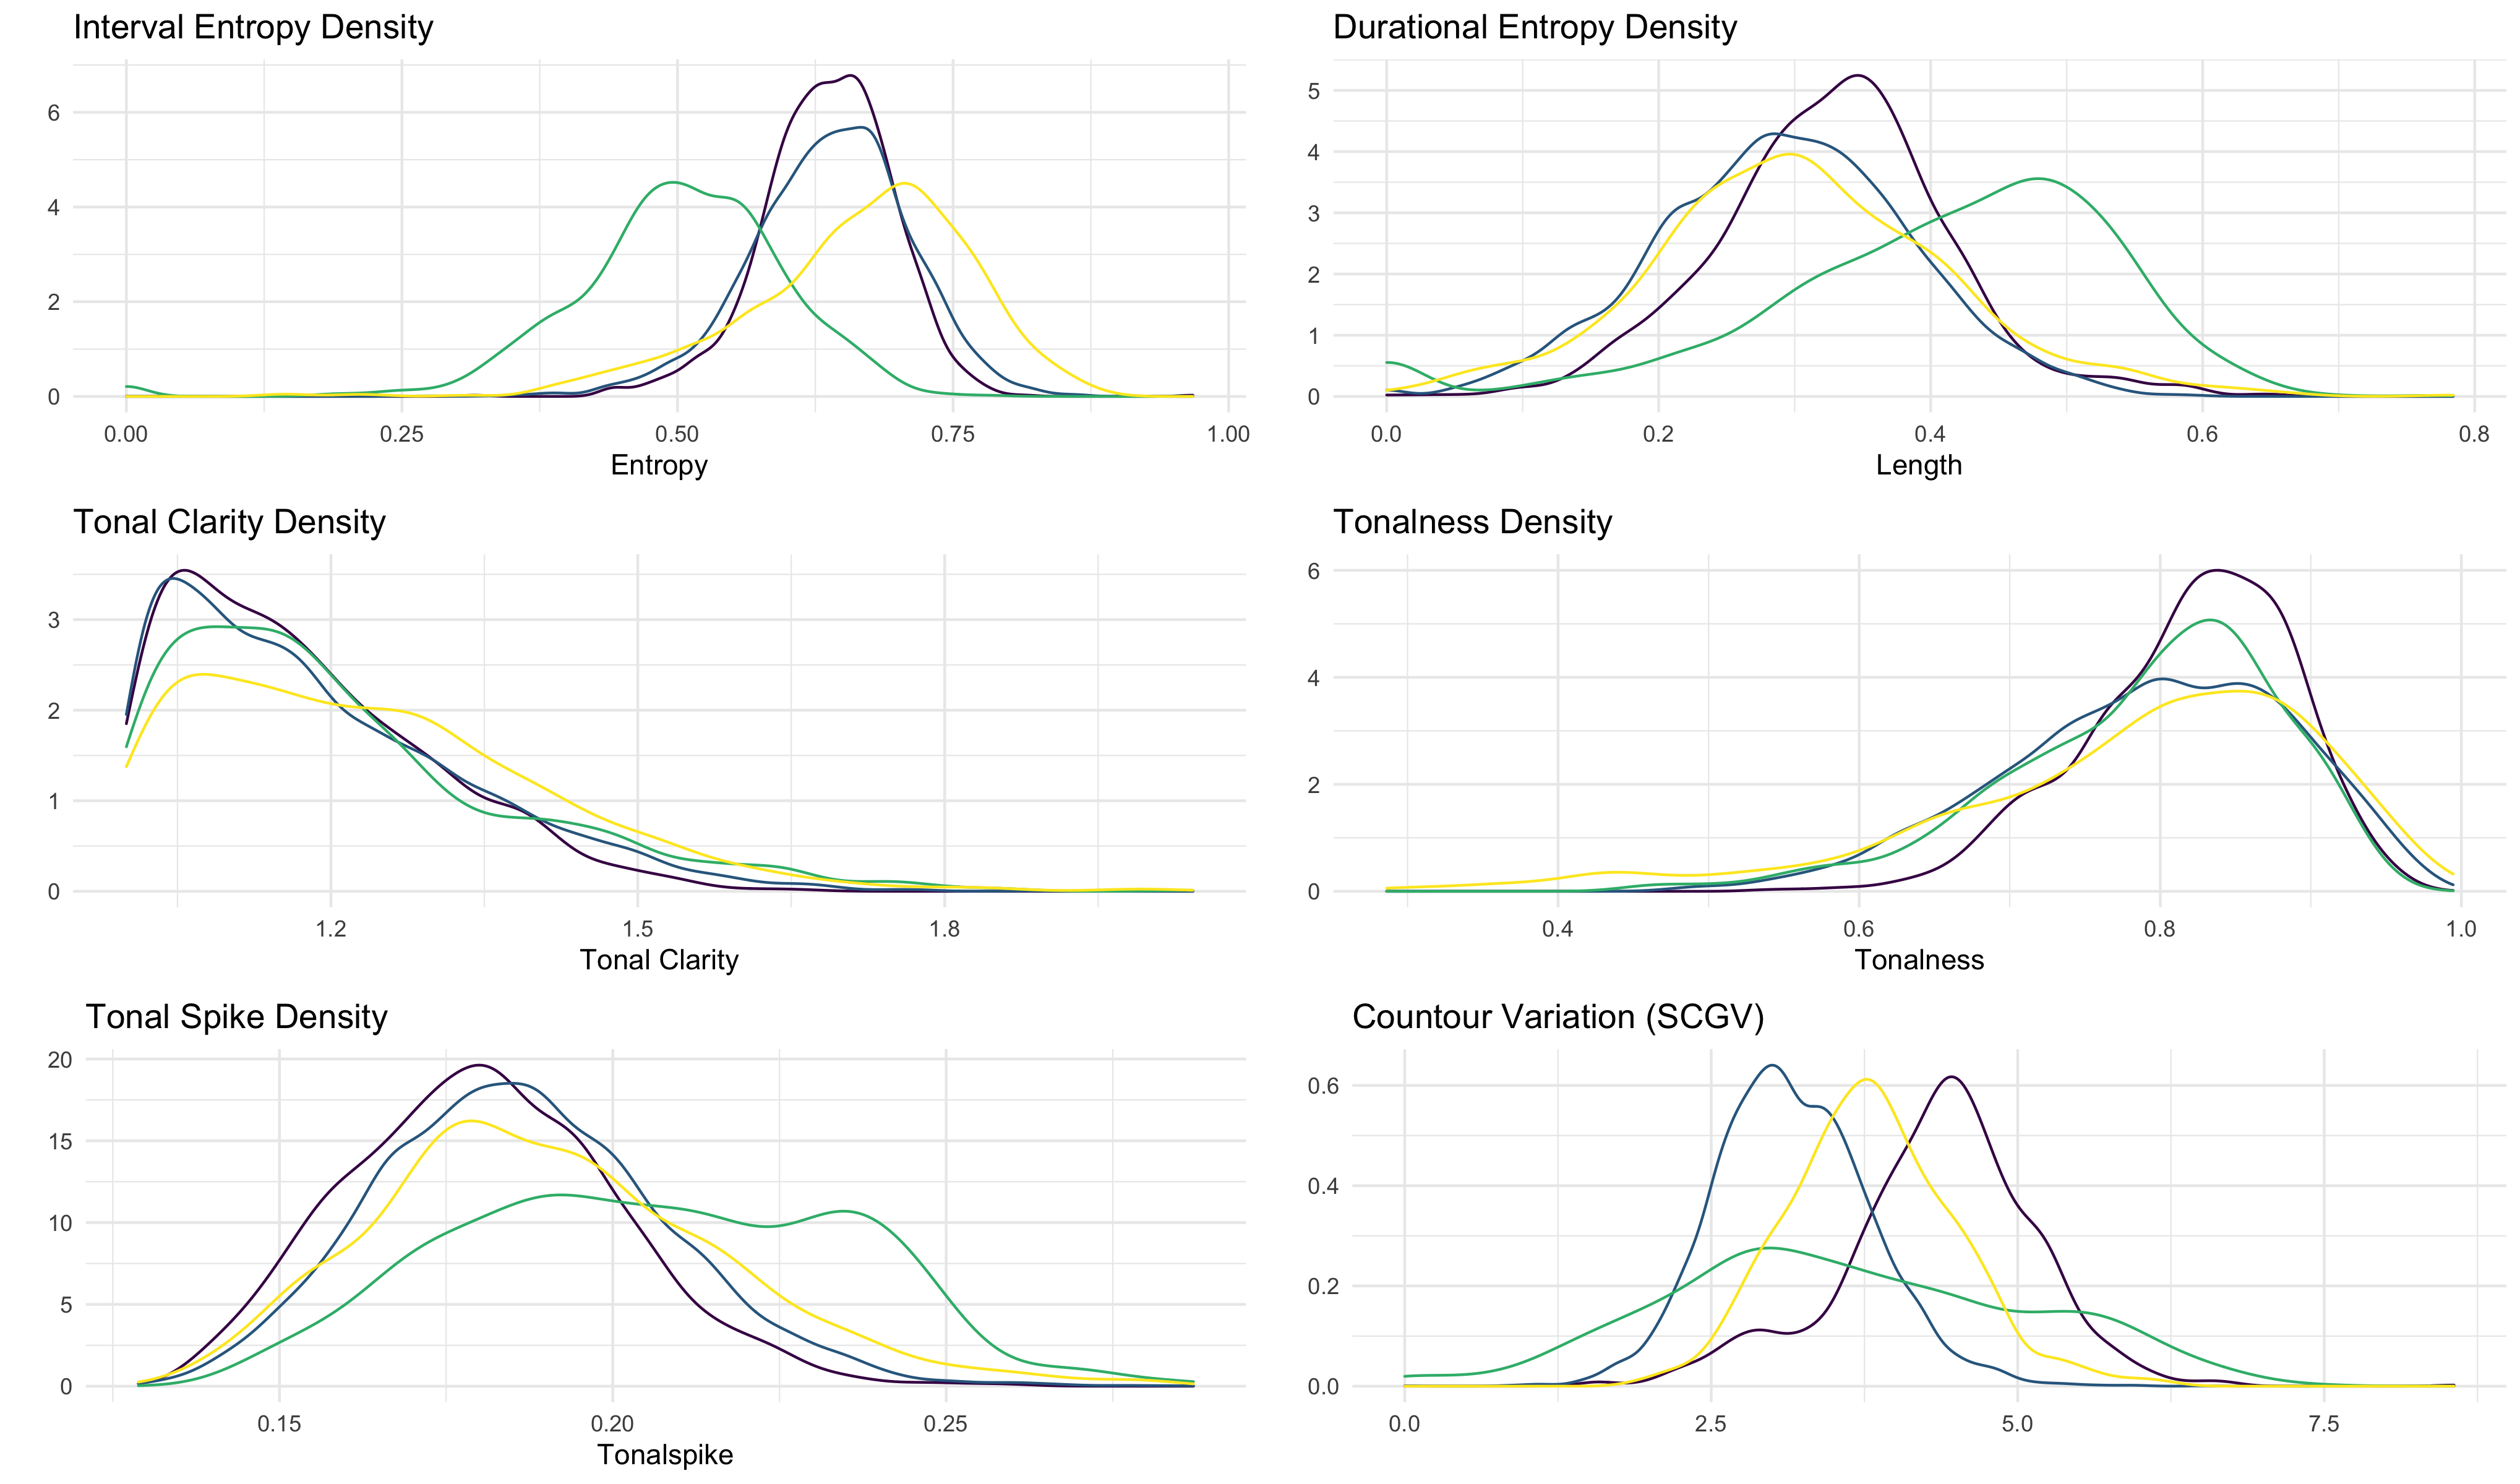
\includegraphics{../img/corpora_emergent.png}
\caption{FANTASTIC Density Plots}
\end{figure}

\begin{figure}
\centering
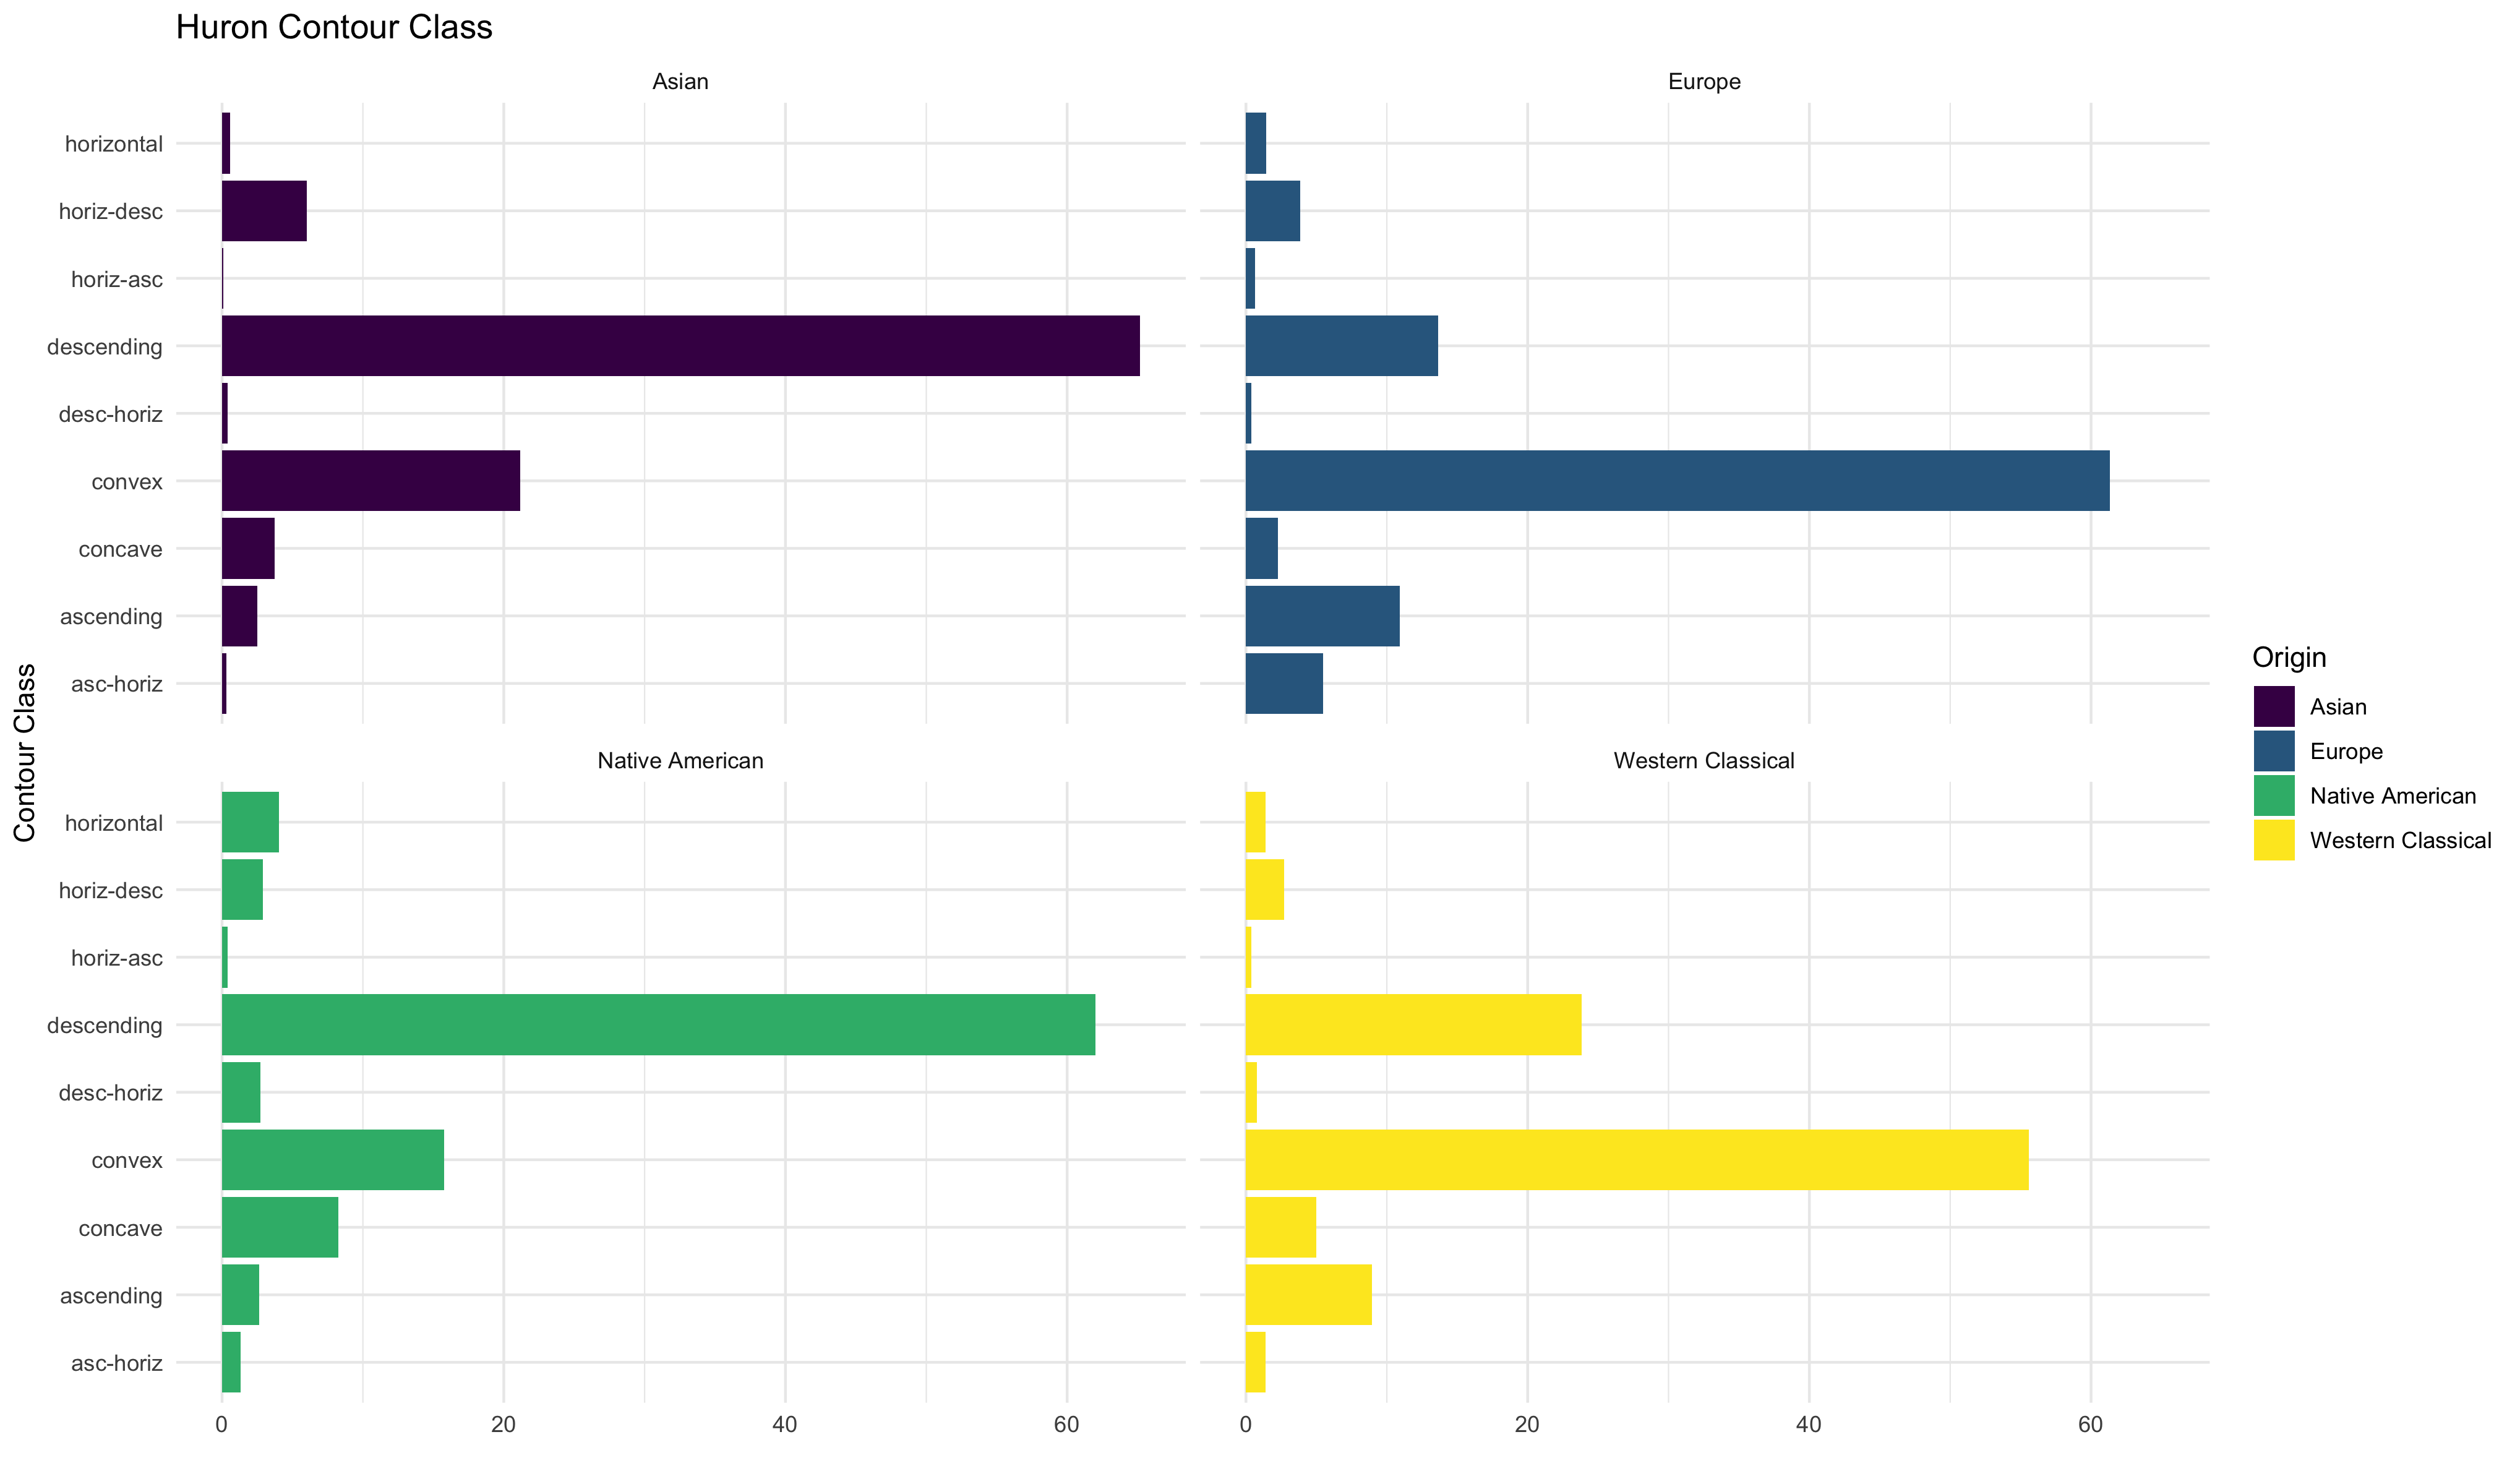
\includegraphics{../img/huron_recreation.png}
\caption{Huron Countour Class}
\end{figure}

\hypertarget{useful}{%
\section{Useful}\label{useful}}

As the \emph{MeloSol} corpus comprises Western, tonal music, this corpora might be utalized in order to continue research investigating empirical claims about about patterns intrinsic to Western, tonal music.
For example claims made by Huron (Huron, 1996) regarding contour class-- initially explored using this dataset by (Baker, 2019)-- could be further modeled using \emph{MeloSol}.
Additionally, as \emph{MeloSol} strictly contains music associated with Western, tonal music, the corpus could be used in further work replacing the \emph{Essen} collection as a dataset in which to train computational models of melodic expectation (Pearce, 2018).
We finally note that as this corpus was initially developed in order to investigate how to make pedagogical improvements in aural skills classrooms, using \emph{MeloSol} for this purpose would be a logical extension to this programme of research (Baker, 2019).

\hypertarget{acknowledgements}{%
\section{Acknowledgements}\label{acknowledgements}}

Ir would like to thank Adam Rosada, Elizabeth Monzingo, and Connor Davis in their help encoding some of the melodies for this corpus.
Additionally, I would like to thank Daniel Shanahan and Craig Sapp for technical support while working with and always learning new things about humdrum.

\newpage

\hypertarget{references}{%
\section{References}\label{references}}

\begingroup
\setlength{\parindent}{-0.5in}
\setlength{\leftskip}{0.5in}

\hypertarget{refs}{}
\leavevmode\hypertarget{ref-albrecht2014statistical}{}%
Albrecht, J. D., \& Huron, D. (2014). A statistical approach to tracing the historical development of major and minor pitch distributions, 1400-1750. \emph{Music Perception: An Interdisciplinary Journal}, \emph{31}(3), 223--243.

\leavevmode\hypertarget{ref-phdthesis}{}%
Baker, D. J. (2019). \emph{Modeling melodic dictation} (PhD thesis). Louisiana State University.

\leavevmode\hypertarget{ref-berkowitzNewApproachSight2011}{}%
Berkowitz, S., Fontrier, G., Kraft, L., Goldstein, P., \& Smaldone, E. (2011). \emph{A new approach to sight singing} (5th ed). New York: W.W. Norton.

\leavevmode\hypertarget{ref-demorest201612}{}%
Demorest, S. M., \& Morrison, S. J. (2016). 12 quantifying culture: The cultural distance hypothesis of melodic expectancy. \emph{The Oxford Handbook of Cultural Neuroscience}, 183.

\leavevmode\hypertarget{ref-huronHumdrumToolkitReference1994}{}%
Huron, D. (1994). The Humdrum Toolkit: Reference Manual. Center for Computer Assisted Research in the Humanities.

\leavevmode\hypertarget{ref-huronMelodicArchWestern1996}{}%
Huron, D. (1996). The Melodic Arch in Western Folk Songs. \emph{Computing in Musicology}, \emph{10}, 3--23.

\leavevmode\hypertarget{ref-huronSweetAnticipation2006}{}%
Huron, D. (2006). \emph{Sweet Anticipation}. MIT Press.

\leavevmode\hypertarget{ref-mullensiefenFantasticFeatureANalysis2009}{}%
Mullensiefen, D. (2009). Fantastic: Feature ANalysis Technology Accessing STatistics (In a Corpus): Technical Report v1.5.

\leavevmode\hypertarget{ref-neubarthSupervisedDescriptivePattern2018}{}%
Neubarth, K., Shanahan, D., \& Conklin, D. (2018). Supervised descriptive pattern discovery in Native American music. \emph{Journal of New Music Research}, \emph{47}(1), 1--16. \url{https://doi.org/10.1080/09298215.2017.1353637}

\leavevmode\hypertarget{ref-pearceStatisticalLearningProbabilistic2018a}{}%
Pearce, M. T. (2018). Statistical learning and probabilistic prediction in music cognition: Mechanisms of stylistic enculturation: Enculturation: Statistical learning and prediction. \emph{Annals of the New York Academy of Sciences}, \emph{1423}(1), 378--395. \url{https://doi.org/10.1111/nyas.13654}

\leavevmode\hypertarget{ref-sappHumdrumExtras2008}{}%
Sapp, C. (2008). Humdrum Extras.

\leavevmode\hypertarget{ref-schaffrathEssenFolkSong1995}{}%
Schaffrath, H. (1995). The Essen Folk Song Collection, D. Huron.

\leavevmode\hypertarget{ref-shanahanDensmoreCollectionNative2014}{}%
Shanahan, D., \& Shanahan, E. (2014). The Densmore Collection of Native American Songs: A New Corpus for Studies of Effects of Geography, Language, and Social Function on Folk Song. In \emph{Proceedings of the Fourteenth Annual International Conference for Music Perception and Cognition}. San Francisco.

\leavevmode\hypertarget{ref-wernerMuseScore2019}{}%
Werner, S., Nicholas, F., \& Bonte, T. (2019). MuseScore.

\endgroup

\end{document}
